% 
% Annual Cognitive Science Conference
% Sample LaTeX Paper -- Proceedings Format
% 

% Original : Ashwin Ram (ashwin@cc.gatech.edu)       04/01/1994
% Modified : Johanna Moore (jmoore@cs.pitt.edu)      03/17/1995
% Modified : David Noelle (noelle@ucsd.edu)          03/15/1996
% Modified : Pat Langley (langley@cs.stanford.edu)   01/26/1997
% Latex2e corrections by Ramin Charles Nakisa        01/28/1997 
% Modified : Tina Eliassi-Rad (eliassi@cs.wisc.edu)  01/31/1998
% Modified : Trisha Yannuzzi (trisha@ircs.upenn.edu) 12/28/1999 (in process)
% Modified : Mary Ellen Foster (M.E.Foster@ed.ac.uk) 12/11/2000
% Modified : Ken Forbus                              01/23/2004
% Modified : Eli M. Silk (esilk@pitt.edu)            05/24/2005
% Modified : Niels Taatgen (taatgen@cmu.edu)         10/24/2006
% Modified : David Noelle (dnoelle@ucmerced.edu)     11/19/2014

%% Change "letterpaper" in the following line to "a4paper" if you must.

\documentclass[10pt,letterpaper]{article}

\usepackage{cogsci}
\usepackage{comment}
\usepackage{pslatex}
\usepackage{apacite}
\usepackage{amsmath,amssymb}
\usepackage{graphicx}
\usepackage{subcaption}
\usepackage{color}
\usepackage{url}
\usepackage{todonotes}
\usepackage{mathtools}
\usepackage{stmaryrd}
\usepackage{booktabs}
\usepackage{array}
\usepackage{caption}
\usepackage{sidecap}
\usepackage{capt-of}
\usepackage{nicefrac}
\usepackage[export]{adjustbox}
\usepackage{makecell}
\hyphenpenalty=100000
\renewcommand\theadfont{\normalsize}
\usepackage[font={footnotesize}]{caption}
\newcommand{\jefan}[1]{{\color{blue}{[jefan: #1]}}}
\newcommand{\kushin}[1]{{\color{orange}{[kushin: #1]}}}
\newcommand\norm[1]{\left\lVert#1\right\rVert}


\title{Semantic structure in communicative drawings}

 
% \author{\begin{tabular}[htbp]{c@{\extracolsep{1em}}c@{\extracolsep{1em}}c@{\extracolsep{1em}}c} \\
% {\large \bf Kushin Mukherjee} & {\large \bf Robert X. D. Hawkins} & {\large \bf Judith E. Fan}\\
% Department of Cognitive Science  & Department of Psychology & Department of Psychology \\ 
% Vassar College & Stanford University & Stanford University \\
% \texttt{kumukherjee@vassar.edu} & \texttt{rxdh@stanford.edu} & \texttt{jefan@stanford.edu} \\
% \end{tabular}
% }

% \author{{\large \bf Kushin Mukherjee\textsuperscript{1}, Robert X. D. Hawkins\textsuperscript{2}, Judith E. Fan\textsuperscript{2,3}} \\
% \textsuperscript{1}Department of Cognitive Science, Vassar College, \\
% \textsuperscript{2}Department of Psychology, Stanford University, \\
% \textsuperscript{3}Department of Psychology, University of California, San Diego}

\author{\large \bf Anonymous Authors}

\begin{document}
\makeatletter
\let\@oldmaketitle\@maketitle% Store \@maketitle
\renewcommand{\@maketitle}{\@oldmaketitle% Update \@maketitle to insert...
  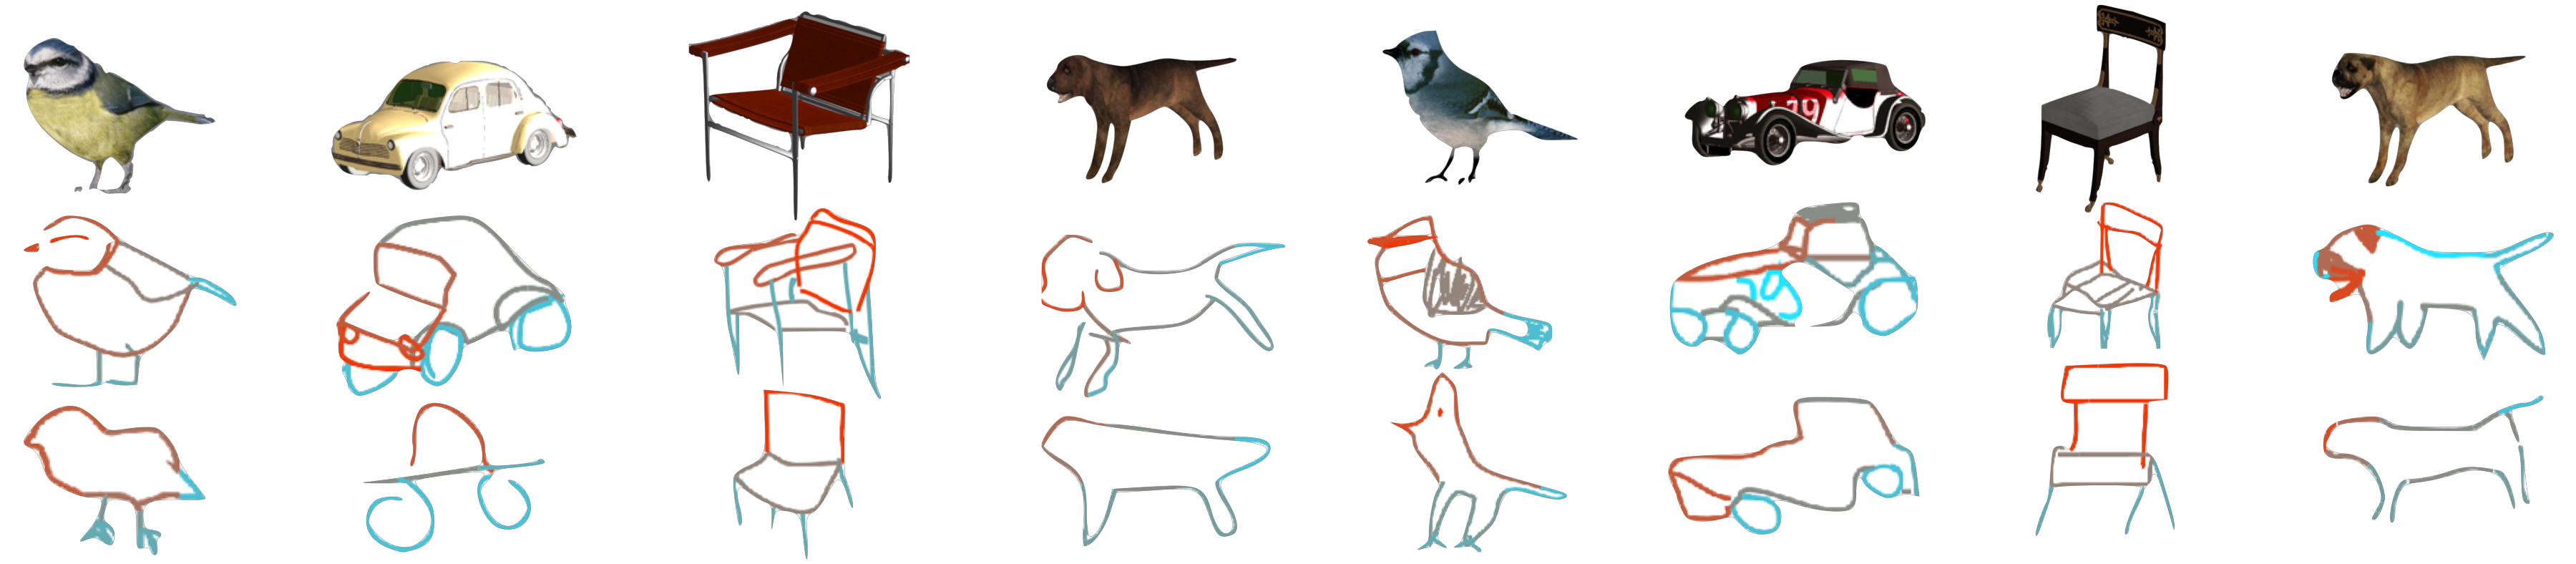
\includegraphics[width=0.95\textwidth]
    {figures/1_banner.pdf}
    \captionsetup{width=0.95\textwidth}
 \captionof{figure}{\footnotesize{Objects used in communication game with example drawings of each object, where stroke color indicates different parts.}}\bigskip}% ... an image
\makeatother

\maketitle 

\begin{abstract}

The ability to represent semantically meaningful structure in our environment is a powerful aspect of human visual perception and cognition. 
As a testament to this ability, we effortlessly grasp the correspondence between a drawing of an object and that physical object in the world, even if the sketch is far from realistic. 
How are visual object concepts organized such that they can robustly encode such abstract correspondences?
Here we consider the possibility that this is in part because we readily decompose both objects and drawings into a common set of semantically meaningful parts. 
To evaluate this, we developed a web-based platform to densely annotate the parts represented in drawings of real-world objects that varied in how detailed they were.  
We found that: \textit{1}, people are highly consistent in how they interpret what individual strokes represent; \textit{2}, single strokes tend to correspond to single parts; \textit{3}, strokes representing the same part tend to be clustered in time during production; and \textit{4}, both more detailed and sparser drawings of the same object emphasized similar part information, although \textit{5}, detailed drawings of different objects tend to be more distinct from one another than sparser ones. 
Taken together, our results support the notion that people deploy their abstract understanding of the compositional part structure of objects in order to select actions to communicate relevant information about them in context. 
More broadly, they highlight the importance of structured knowledge for understanding how pictorial representations convey meaning. 

\textbf{Keywords:} 
sketch understanding; perceptual organization; visual production; compositionality; objects and categories
\end{abstract}

\section{Introduction}

%% revise so that the throughline is clearer: how does the human mind organize visual concepts such that they can be deployed so flexibly? answer: compositionality. what is a good way of probing compositionality? you could use discrimination tasks, but compositional tasks are much more direct. what is good about compositionality? it enables flexibility. how do you probe flexibility? compositional tasks across different contexts. 

When we open our eyes, we do not experience a meaningless array of photons --- instead, we parse the world into people, objects, and their relationships. 
The ability to represent semantically meaningful structure in our environment is a core aspect of human visual perception and cognition \cite{navon1977forest}. 
As a testament to this ability, we effortlessly grasp the correspondence between a sketch of a particular object and that physical object in the world, even if the sketch is far from realistic \cite{eitz2012humans,FanCommon2018}. 
How are visual object concepts organized such that they can robustly encode such abstract correspondences?
Here we explore the hypothesis that this is in part because we readily decompose both objects and drawings into a common set of semantically meaningful parts \cite{biederman1988surface}. 

Recent advances in computational neuroscience and artificial intelligence have provided an unprecedentedly clear view into the algorithms used by the brain to extract semantic information from raw visual inputs, exemplified by modern deep learning approaches \cite{yamins2014performance}.
Nevertheless, a major gap remains in elucidating how the feature representations learned by deep learning models can be adapted to emulate the structure and flexibility of human visual semantic knowledge \cite{lake2017building}.
A promising approach to closing this gap may be to combine the learning capacity of deep neural networks with the parsimony and interpretability of structured representations that reflect how visual concepts are organized in the mind \cite{battaglia2018relational}. 
However, pursuing this strategy relies on a thorough understanding of this conceptual organization and how this organization enables behavioral flexibility.  

The goal of this paper is to contribute to this understanding by probing the expression of visual semantic knowledge in a naturalistic setting that exposes both its structure and flexibility: visual communication via drawing. 
This approach departs from the conventional strategy for inferring the organization of visual object concepts from behavior, which relies upon tasks that elicit judgments about visual inputs, usually with respect to experimenter-defined dimensions. 
By contrast, visual communication tasks permit participants to include any elements they consider relevant to their goals and combine these elements freely, yielding high-dimensional information about how visual semantic knowledge is organized and deployed under a naturalistic task objective. 

Our aim in probing the semantic structure of communicative drawings is to shed light on how the semantic organization of visual object representations supports their flexible expression across contexts. 
Our approach advances recent work \cite{FanCommon2018} that has investigated the production of object drawings to communicate in two ways: first, an explicit focus on compositional semantic structure in drawings, and second, the examination of flexibility in how visual semantic knowledge is expressed in different semantic contexts. 

Towards this end, we developed a web-based platform to densely annotate drawings of real-world objects produced in different semantic contexts, including detailed and simpler drawings of each object. 
Overall, we found that: (1) people are highly consistent in how they interpret what individual strokes represent; (2) single strokes tend to correspond to single parts; (3) strokes representing the same part tend to be clustered in time; and (4) detailed and sparse drawings of the same object emphasized similar part information, although (5) detailed drawings of different objects tend to be more distinct from one another than simpler ones. 
Taken together, our results support the notion that people deploy their abstract understanding of the compositional part structure of objects in order to select actions to communicate relevant information about them in context. 

\section{Methods}

\begin{figure}[htbp]
\centering
\includegraphics[width=0.48\textwidth]{figures/2_refgame_performance.pdf}
\caption{(A) drawings were collected in the context of a two-player drawing-based reference game in which one participant (drawer) aimed to draw a target object so that the other participant (viewer) could distinguish it from three distractor objects. (B) In close contexts, the target and distractors all belonged to the same basic-level category; in far contexts, the target and distractors belonged to different basic-level categories. (C) Drawers used fewer strokes in the far condition, while producing drawings that were accurately recognized by the viewer in both conditions.}
\label{refgame_performance}
\end{figure}

\subsection{Communicative drawing dataset}
We obtained 1195 drawings of 32 real-world objects from a recent experimental dataset in which participants were paired in an online environment to play a drawing-based reference game \cite{fan2018modeling}.\footnote{All materials and data will be made available following the completion of the review process.}
% \footnote{All materials and data are available at \url{https://github.com/cogtoolslab/semantic_parts}.}
Objects belonged to one of four basic-level categories (i.e., bird, car, chair, dog), each of which contained eight exemplars. %(Fig.~\ref{refgame_gallery}A).
On each trial of this reference-game experiment, both participants were presented with a shared context containing an array of photorealistic 3D renderings of four objects.   
One participant (i.e., the drawer) aimed to draw one of these objects -- the target -- so that the other participant (i.e., the viewer) could pick it out from a set of distractor objects (Fig.~\ref{refgame_performance}A). 
Across trials, the similarity of the distractors to the target was manipulated, yielding two types of communicative contexts: close contexts, where the target and distractors all belonged to the same basic-level category, and far contexts, where the target and distractors belonged to different basic-level categories (Fig.~\ref{refgame_performance}B). 
This context manipulation led drawers to produce simpler drawings containing fewer strokes and less ink on far trials than on close trials, while still achieving high recognition accuracy in both types of context (Fig.~\ref{refgame_performance}C). %, Fig.~\ref{refgame_gallery}B\&C). 
 
% \begin{figure*}
% \centering
% 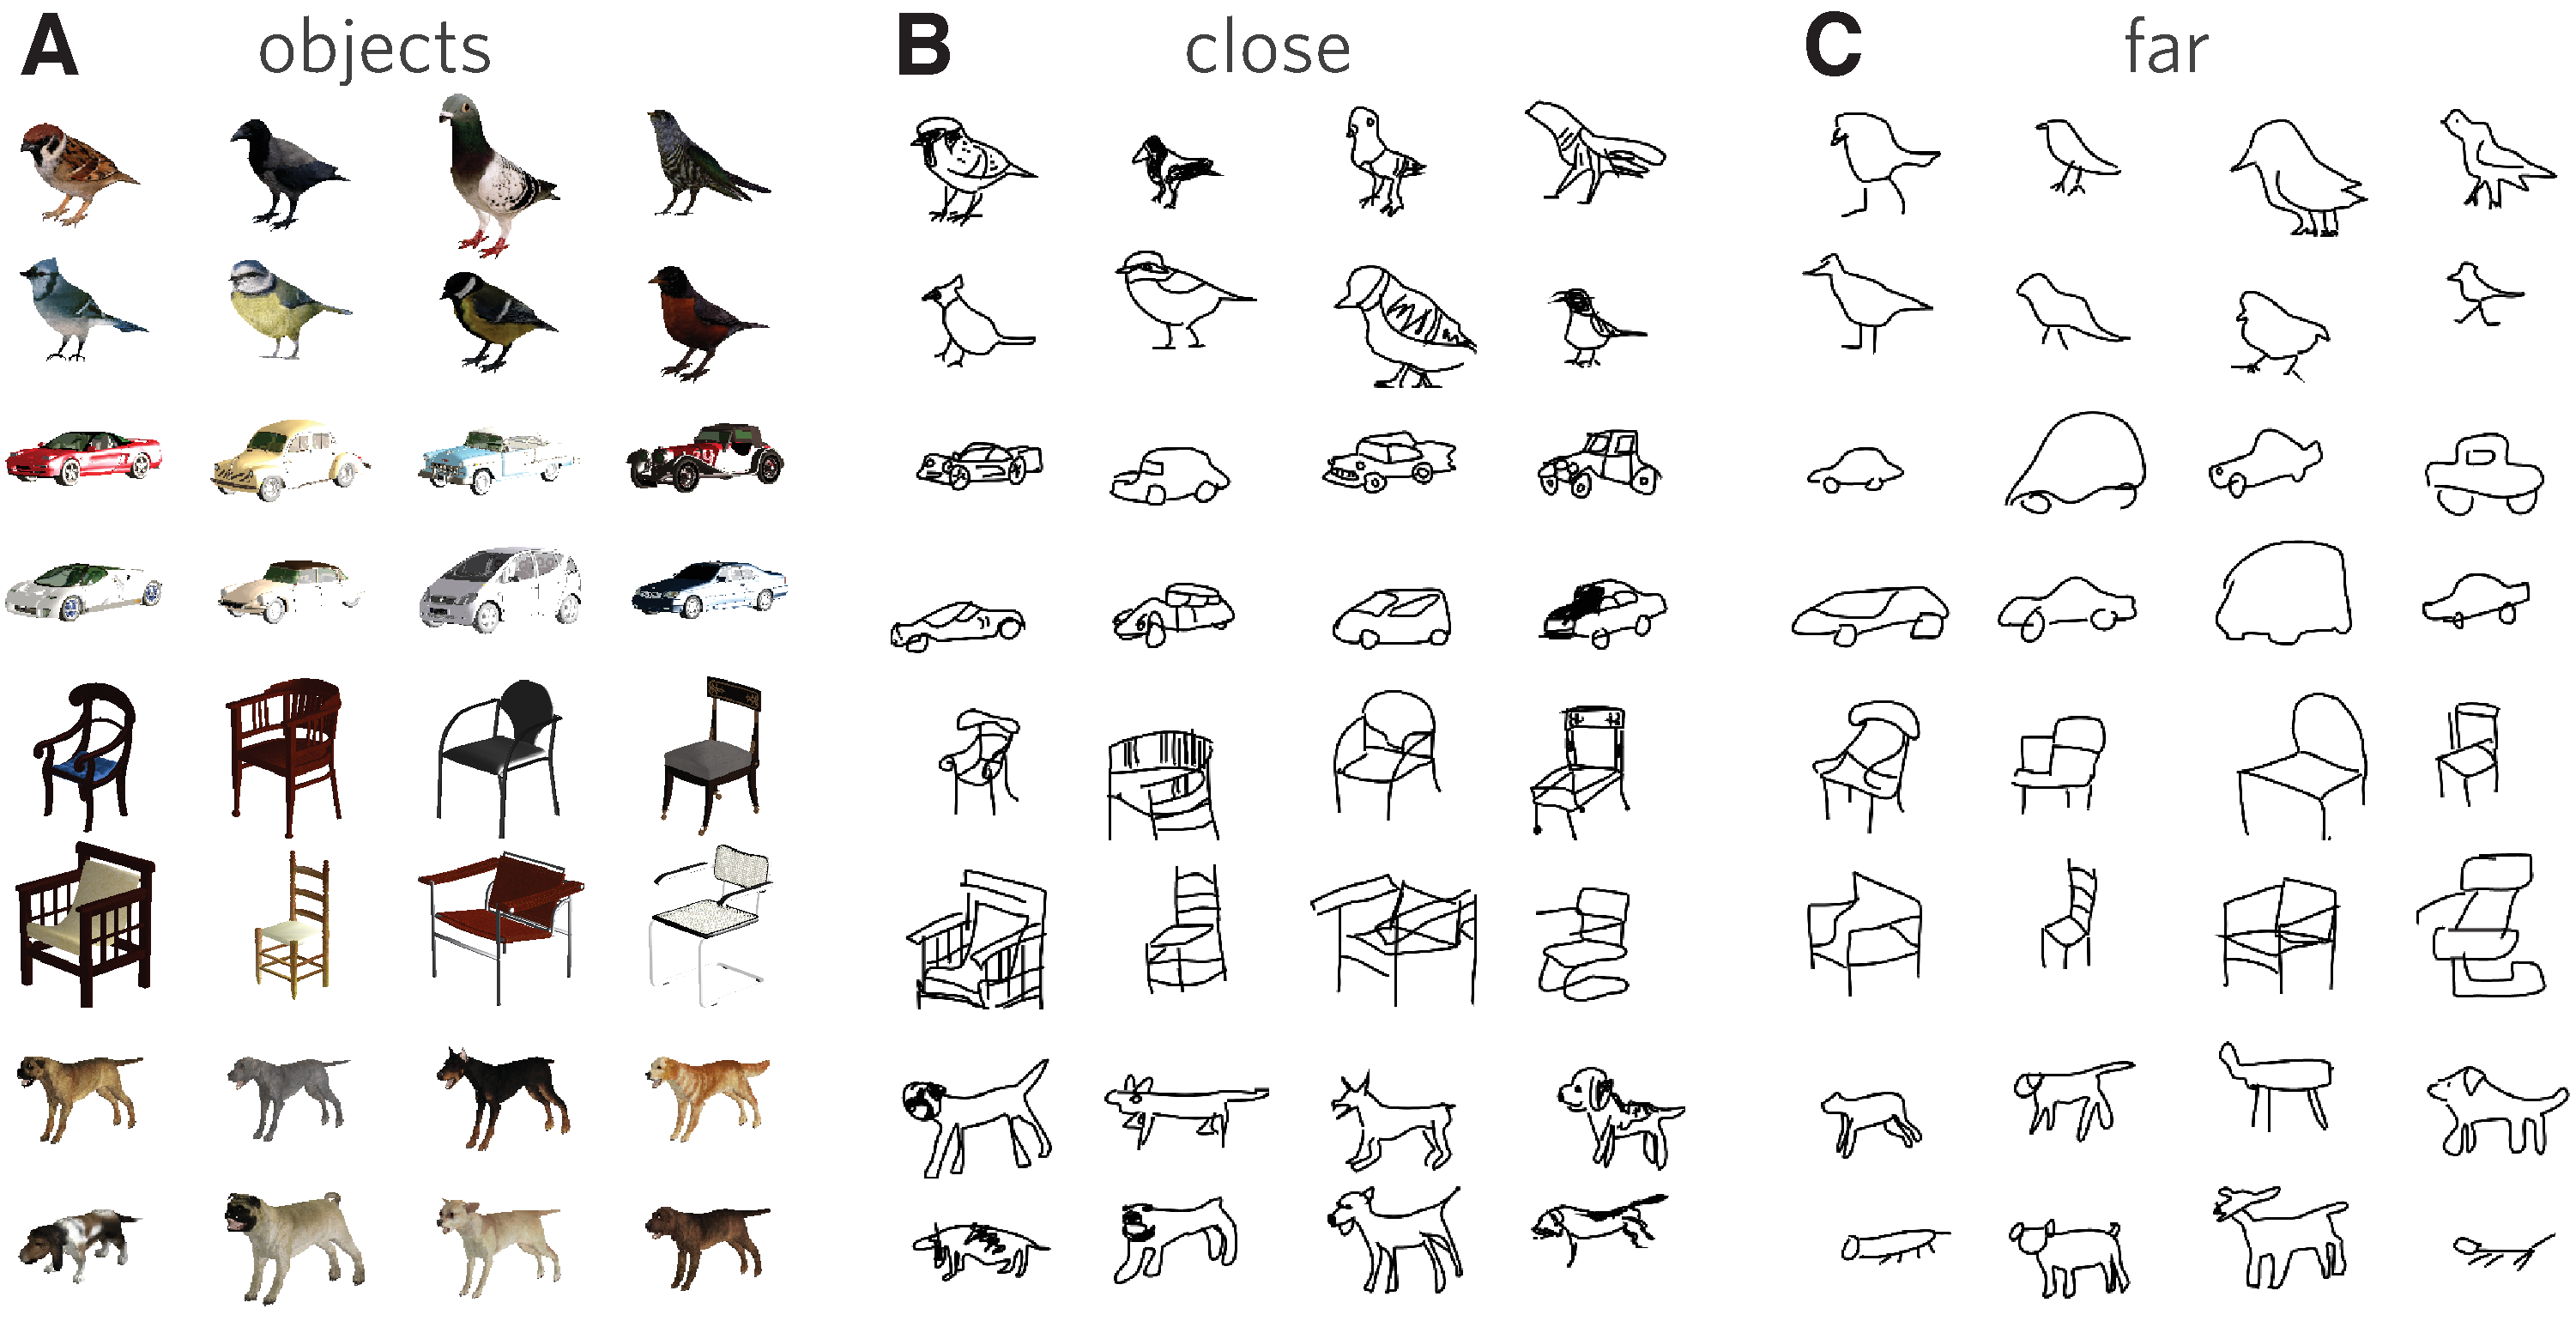
\includegraphics[width=0.95\textwidth]{figures/3_refgame_gallery.pdf}
% \caption{(A) Target objects. (B) Example object drawings produced in a close context. (C) Example drawings produced in a far context.}
% \label{refgame_gallery}
% \end{figure*}


Prior work analyzing the semantic properties of such drawing data have represented them as raster images (e.g., \texttt{*.png}), an expedient format for applying modern convolutional neural network architectures \cite{FanCommon2018,sangkloy2016sketchy,yu2017sketch}. 
However, a key limitation of representing a drawing only as an image is loss of information about the inherently sequential and contour-based nature of drawing production. 
Because our goal was to characterize how semantic structure manifests during drawing production, it was important to encode each drawing instead using a vector image format that preerves this sequential and contour information (i.e., \texttt{*.svg}). 

Each drawing in our dataset is represented as a sequence of individual strokes, where each stroke consists of a sequence of sub-stroke elements, known as splines. 
These splines are parameterized as cubic Bezier curve segments, which are uniquely defined by four points: the initial point, the final point, and two control points that control the spline's curvature.
This data format provides a relatively compact representation of each drawing compared with a rasterized image, while still providing sufficient expressivity to provide an accurate representation. 

\subsection{Semantic part annotation}

Here we developed a novel web-based platform to crowdsource semantic annotations for every spline of every stroke of communicative drawings in our dataset. 

\subsubsection{Participants}
326 participants were recruited via Amazon Mechanical Turk (AMT) and provided informed consent in accordance with the Stanford University IRB. 
Participants were provided with a base compensation of \$0.35, plus \$0.002 for every spline they annotated and \$0.02 for every sketch they annotated completely. 

\subsubsection{Task}
Participants were presented with 10 drawings that were randomly sampled from the reference-game dataset. 
Each trial, one of these drawings appeared in the center of the display, above the same array of four objects that the original drawer had viewed, with one of these objects highlighted as the target (Fig.~\ref{annotation_interface}). 
Thus the participant had full information about which object the drawer had intended to depict, as well as the identity of the distractors. 
Their goal was to tag each spline with a label corresponding to the part it represented (e.g., seat, leg, back for a chair). 
To facilitate this, participants were provided with a menu of common part labels that were associated with each basic-level category represented in our dataset. 
Once a spline was successfully tagged, it was rendered in the color that the part label was associated with in the part menu. 
However, participants could also generate their own part label if none of the common labels applied.
In total, we collected 3608 annotation trials of 1195 unique drawings.

\subsubsection{Data preprocessing}

To avoid bias when analyzing the relative emphasis that drawers placed on different part information, we restricted our analyses to annotation trials in which the sketch was completely annotated (i.e., all splines were tagged). 
Moreover, to evaluate inter-annotator reliability, we only examined drawings that were annotated by at least three distinct participants. 
Some of the custom part labels provided by participants were valid, but at a finer grain than or synonymous to other more frequently occurring labels. 
For example, sometimes strokes that represented subparts of the leg of a chair were labeled as `leg support', `foot', and `strut.'
In order to ensure that parts of drawings were segmented at a consistent level of granularity, we manually constructed a part dictionary to map these overly fine-grained part labels to one of the common part labels. 
After applying these preprocessing steps, our annotated dataset consisted of 864 drawings that had been annotated exactly 3 times each, using a set of 24 unique part labels. 

\begin{figure}[htbp]
\centering
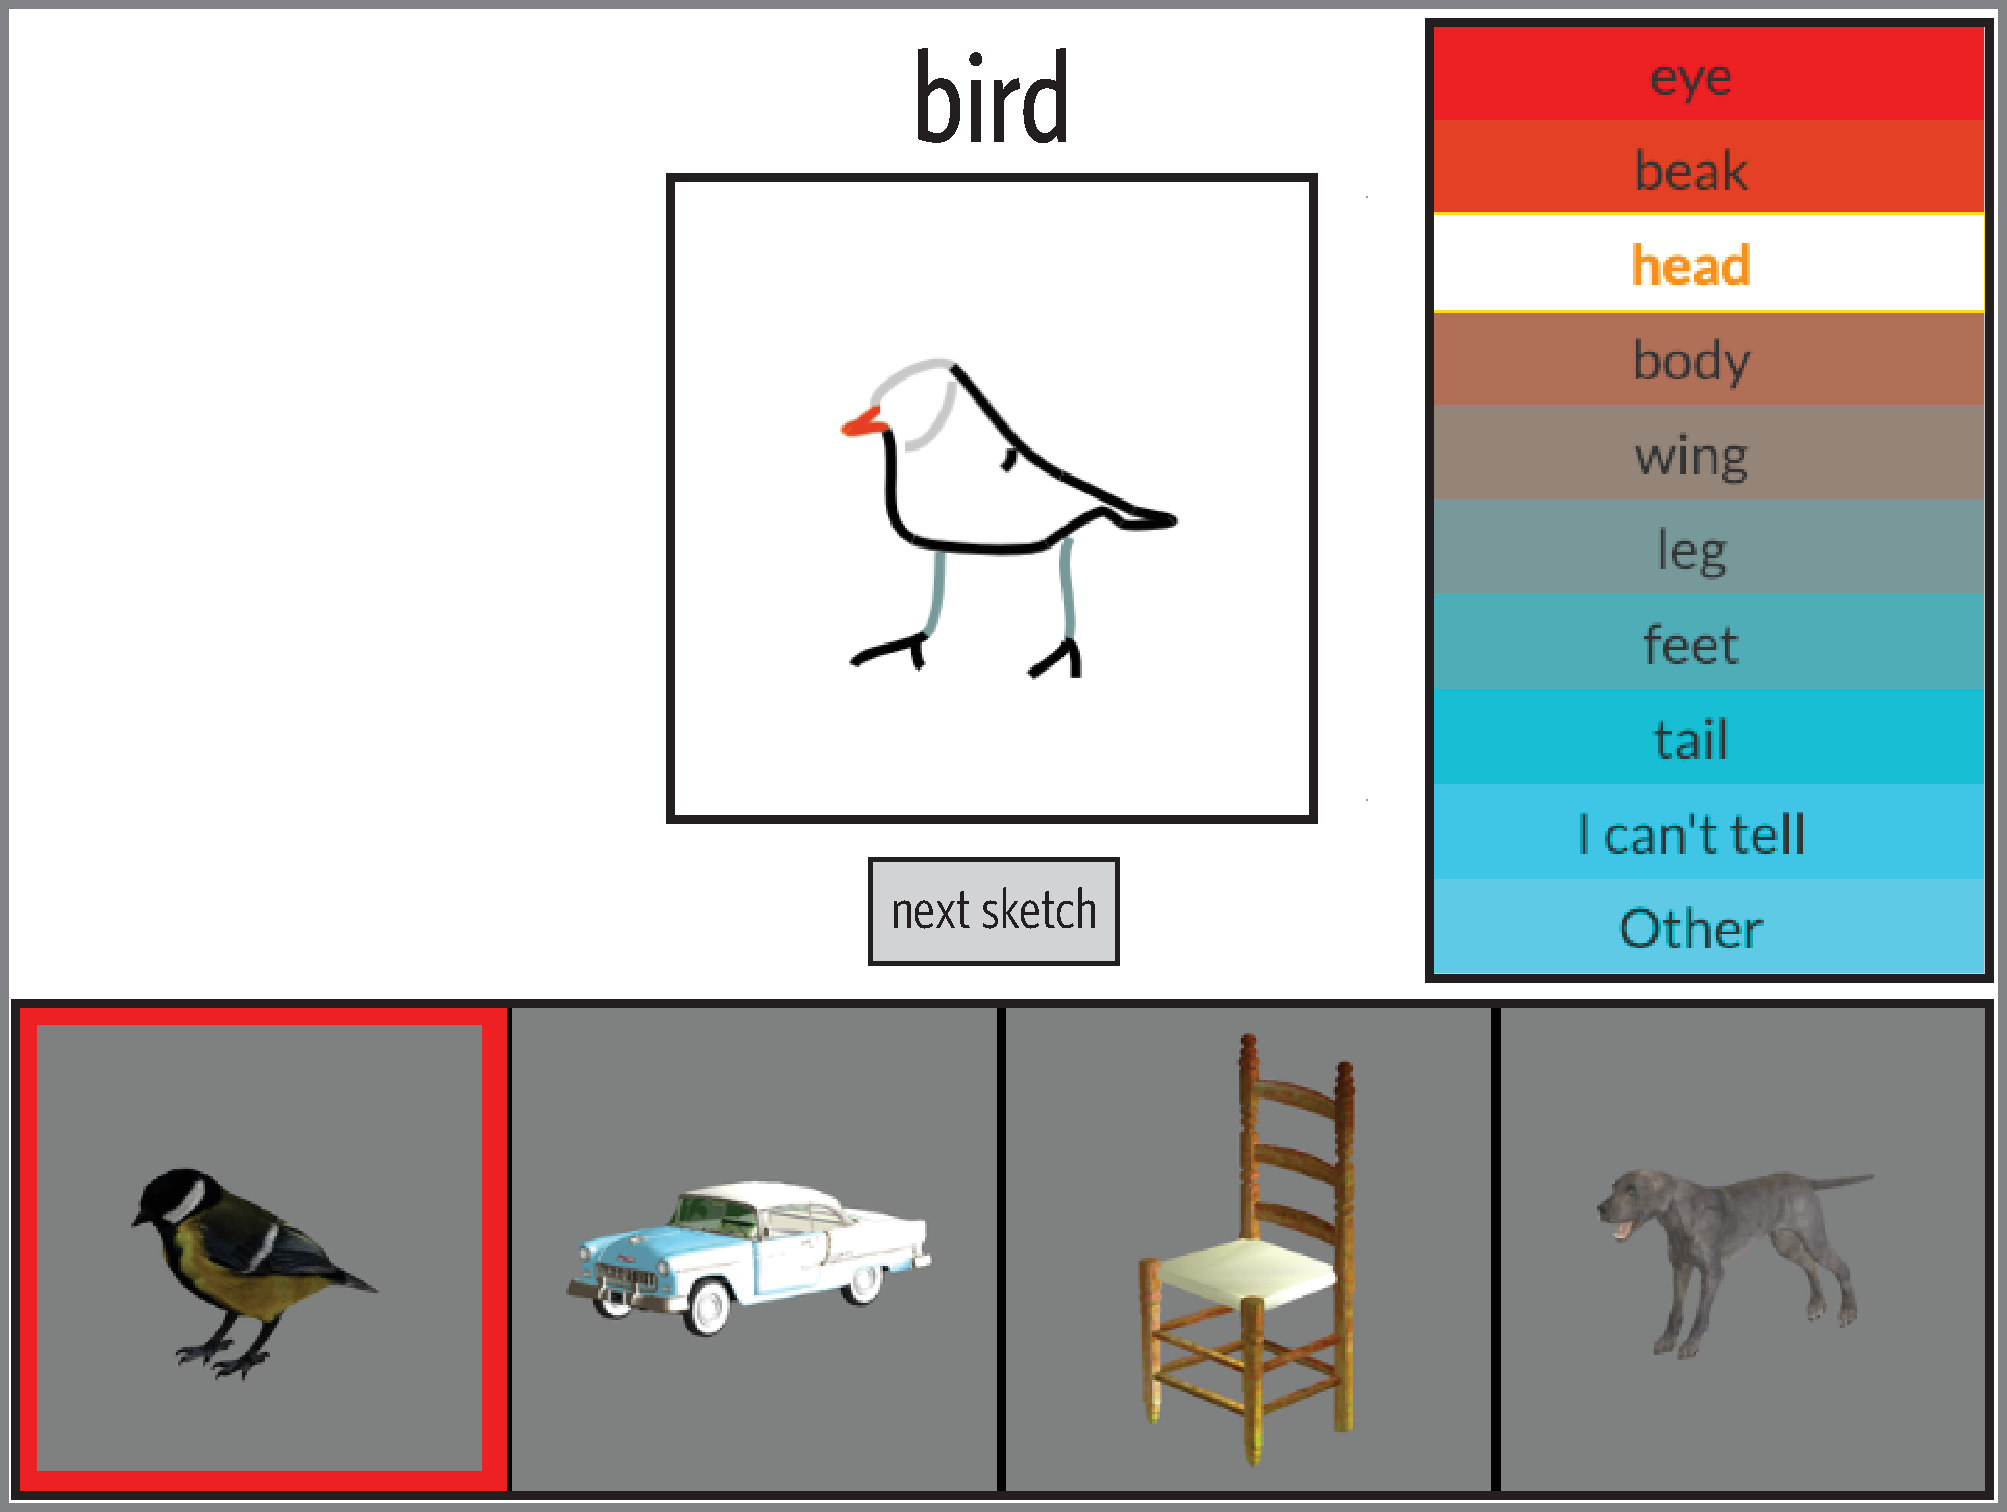
\includegraphics[width=0.48\textwidth]{figures/4_annotation_interface.pdf}
\caption{Sketch annotation interface. Participants selected sub-stroke elements of the sketch and tagged them with category-congruent part labels from the menu. The original communicative context in which the sketch was generated was also provided: the target object (highlighted in red) and three distractors were displayed in an array below the sketch.}
\label{annotation_interface}
\end{figure}

\begin{table}[]
\begin{tabular}{ll}
\hline
\textbf{category} & \textbf{part labels} \\ \hline
bird & eye, beak, head, body, wing, leg, feet, tail \\ \hline
car & \begin{tabular}[c]{@{}l@{}}bumper, headlight, hood, windshield, \\ window, body, door, trunk, wheel\end{tabular} \\ \hline
chair & backrest, armrest, seat, leg \\ \hline
dog & eye, mouth, ear, head, neck, body, leg, paw, tail \\ \hline
\end{tabular}
\caption{Part labels provided to annotators. All user-generated labels were mapped to this set of labels.}
\end{table}


\section{Results}

\subsection{How well do different people agree on what strokes represent?}

Perhaps one of the most basic questions our dataset is poised to answer is how often different viewers agreed on what each stroke element in a sketch represented. 
We found that 95.6\% of all splines in our dataset were given the same label by at least two of the three annotators, with 67.8\% of all splines exhibiting complete agreement among all three annotators. 
This suggests that there is a high degree of consistency in how people decompose drawings into semantically meaningful parts. 
In subsequent analyses, we collapsed over inter-annotator variation: we assigned the modal label to splines to which at least two annotators had given the same label; for the remaining 4.4\% of splines, we sampled one of the three labels provided.

\subsection{How strongly do strokes correspond to parts of objects?}

When composing a recognizable sketch of a real-world object, how do people decide what information to convey with each stroke? 
A natural possibility is that there exists a close correspondence between the actions they perform and their knowledge of what parts that object possesses and how these parts are related to each other.
Concretely, we hypothesized that for most strokes in our dataset, that all sub-stroke elements (splines) would be assigned the same part label. 
However, because the part labels we considered could reasonably apply to multiple sub-parts (e.g., multiple legs on a bird, chair, or dog), we further hypothesized that multiple strokes would frequently be used to represent all instances of that part in a single sketch.

To evaluate the first prediction, we determined how many unique part labels were represented across all sub-stroke elements within each stroke (Fig.~\ref{stroke_to_part}B). 
We found that there was only one part label associated with 81.6\% of the strokes in our dataset, showing that when participants decided to  ss. produced a stroke, most of the time it represented no more than one part of that object. 
18.4\% of strokes were associated with two or more labels, showing that there are still cases where a single stroke may still be used to represent more than one part (e.g., a single stroke connecting the head and body of a bird, or an armrest and leg of a chair). 
This was slightly more common in drawings produced in far contexts (19.4\%, 95 \%CI = 17.9\%, 20.9 \%) than close contexts (17.6\%, 95\% CI : [16.1\%, 18.8\%]).  This might indicate that a candidate strategy for creating sparser abstract drawings may be to utilize individual strokes to represent multiple spatially contiguous parts. 

\begin{figure}[htbp]
\centering
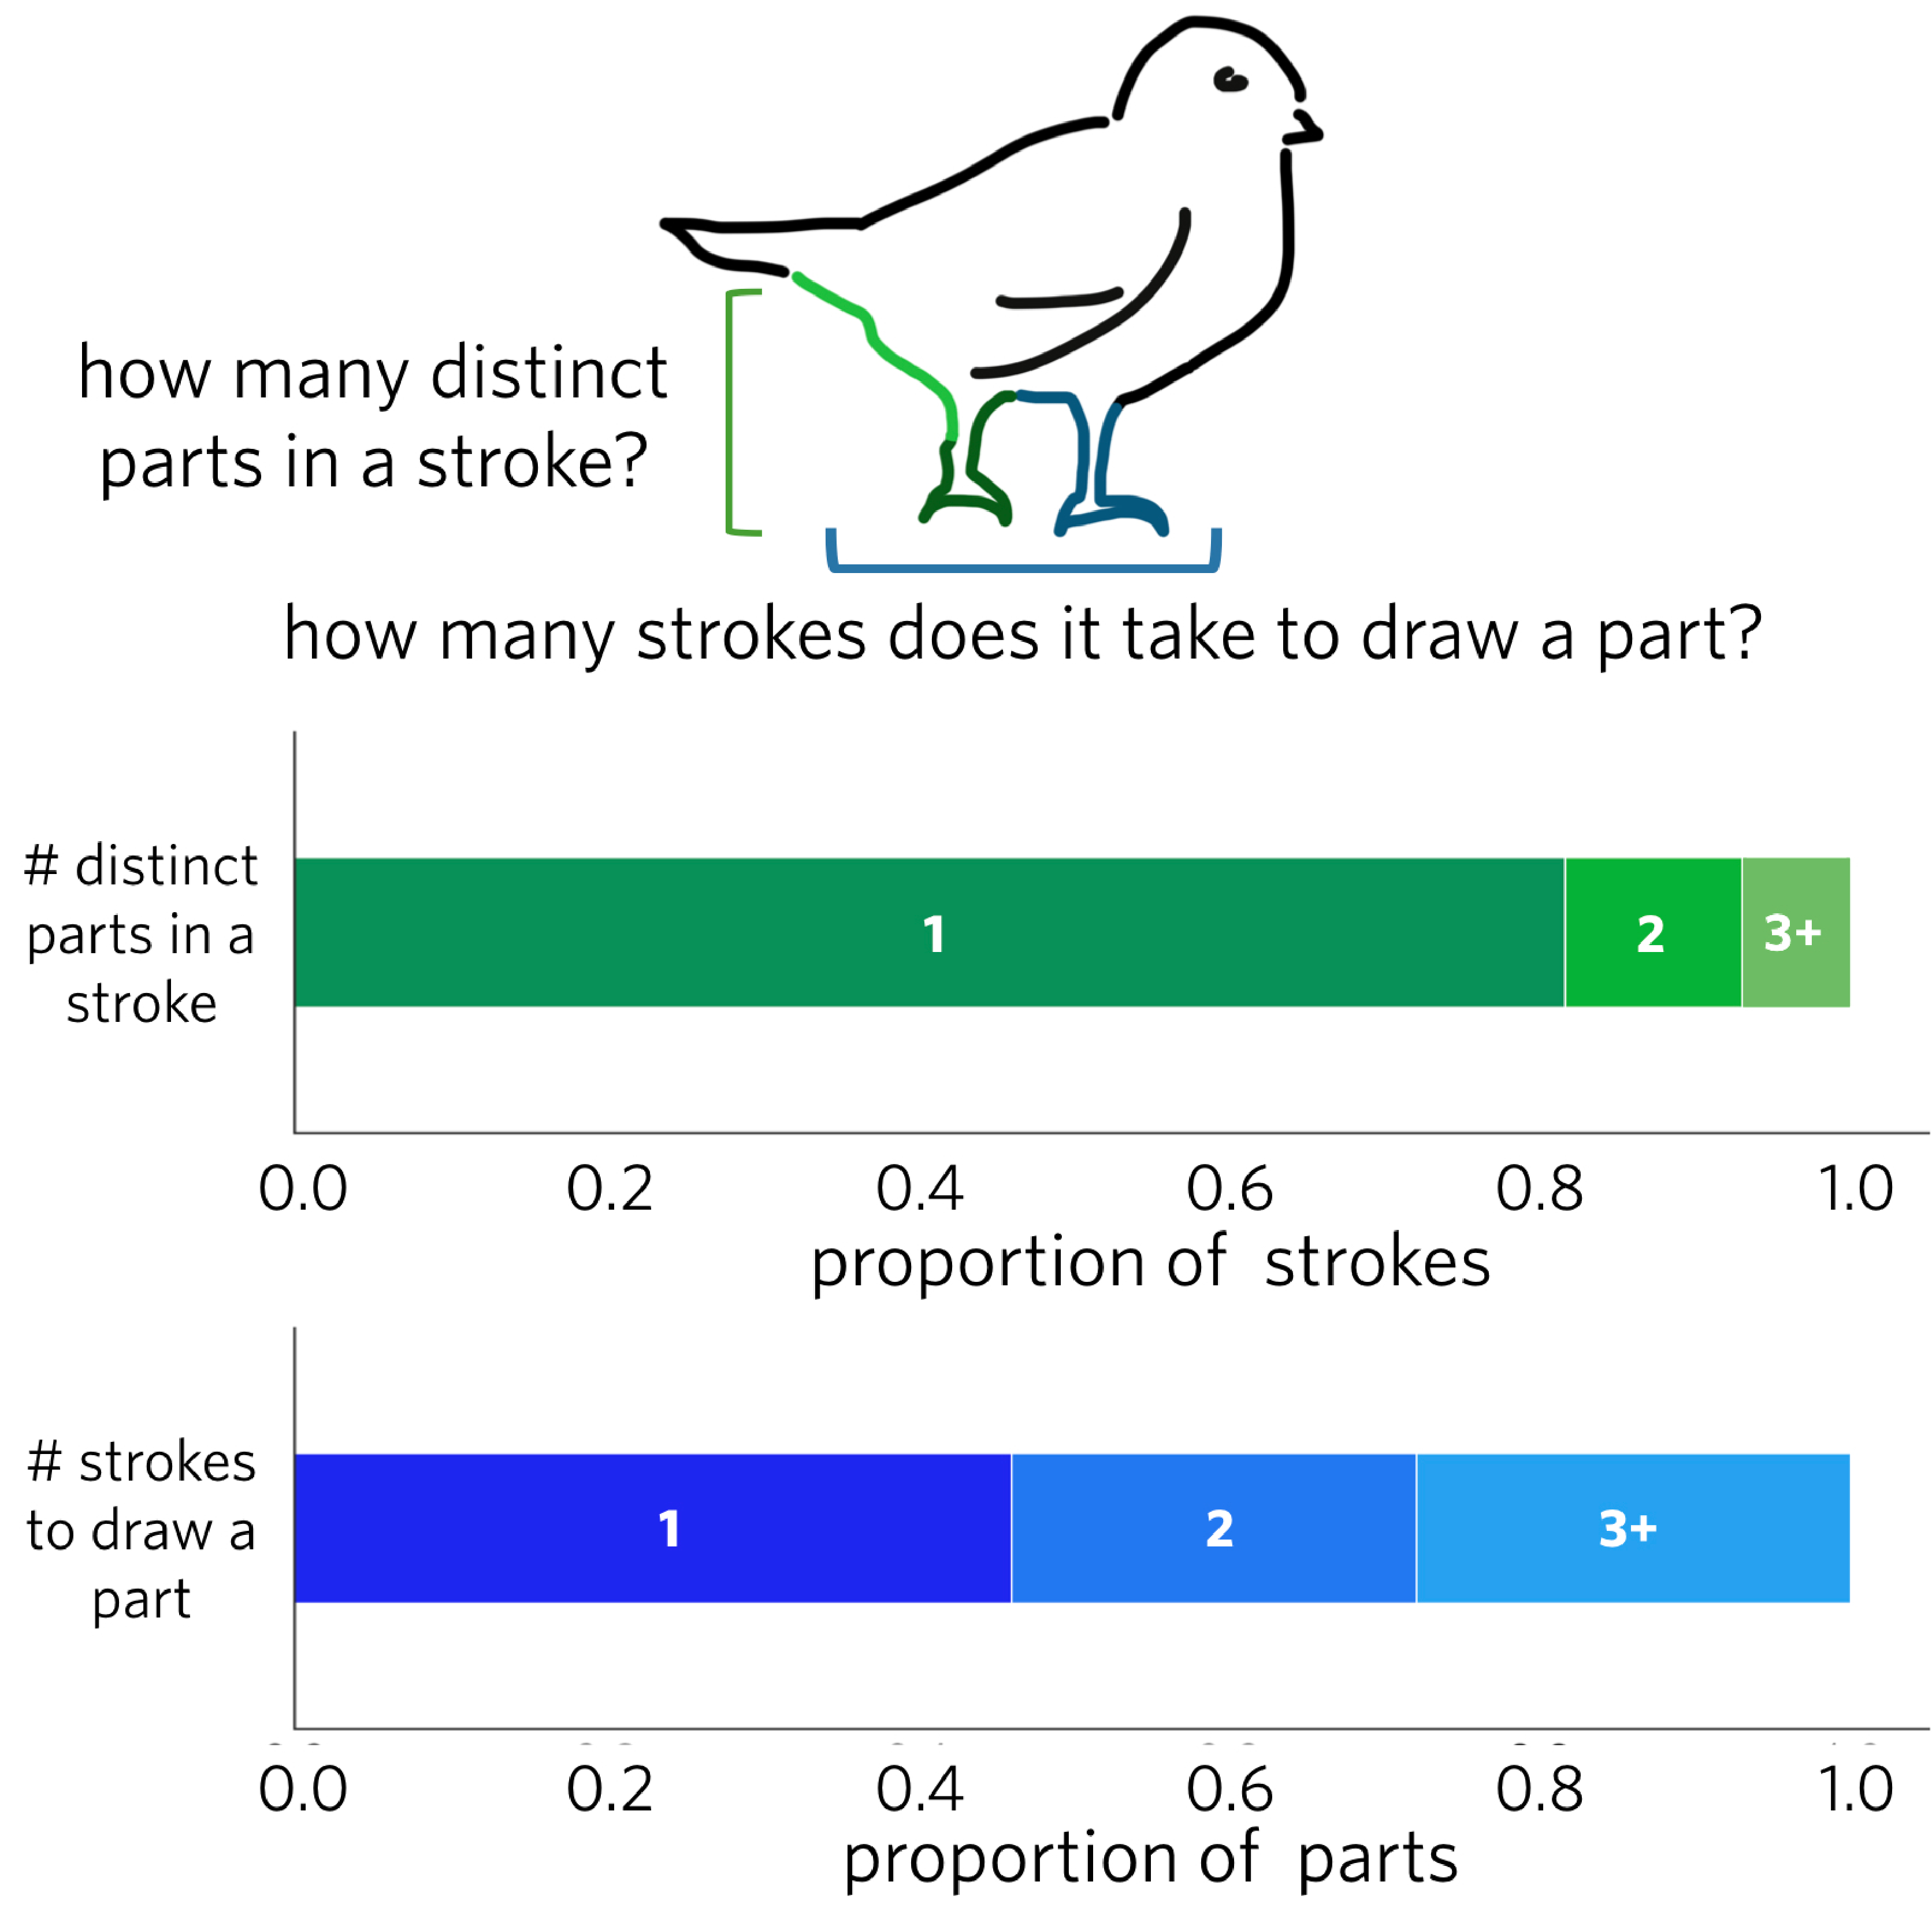
\includegraphics[width=0.48\textwidth]{figures/5_stroke_part_relationship.pdf}
\caption{Correspondence between strokes and part labels. (A) We examined the number of unique labels assigned to the constituent splines of every stroke in our dataset. We also counted how many strokes shared a given part label in every sketch. (B) The majority of strokes contained only a single part label. (C) Almost half the parts across all drawings required only a single stroke to be represented. The remaining parts required at least 2 strokes to be fully represented. }
\label{stroke_to_part}
\end{figure}

To evaluate the second prediction, we determined how many strokes were used to represent each part of an object (Fig.~\ref{stroke_to_part}B). 
We found that 46.1\% of parts were depicted using exactly one stroke, 26.0\% using exactly two strokes, 11.3\% using exactly three strokes, 16.6\% using four or more strokes. 
This shows that nearly half the time, a single action was required to depict an entire object part. 
However, the remaining 53.9\% of parts required more than one stroke to depict, owing to those parts that consisted of multiple disconnected subparts within an object (e.g., wheels of a car, paws of a dog).
\jefan{This should be verified in some way by subsetting on those feature columns that actually are likely to contain multiple instances per object.}
The proportion of parts requiring more than one stroke was slightly higher for close drawings (55.8\%, 95\% CI: [53.7\%, 58.6\%]) than far drawings (52.0\%, 95\% CI: [49.9\%, 54.6\%]), perhaps reflecting the tendency to include more object-diagnostic detail when depicting each part. 

Overall, these findings suggest that when people have the goal of communicating the identity of an object in a drawing, the information they choose to convey with each stroke is far from arbitrary, but rather is tightly coupled to the compositional part structure of objects. 

\subsection{How often are strokes representing the same part produced in succession?}

In the previous section we discovered that for slightly more than half of the parts in each object, more than one stroke was used to depict it. 
This raised the question: to what extent are these multiple strokes depicting the same part being drawn in succession, or being interleaved among strokes corresponding to other parts?

%To investigate this, we estimated the mean length of part streaks consisting of strokes depicting the same part, and compared this to the mean streak length for permuted stroke sequences. 
%We used mean streak length as a proxy for the prevalence of same-part strokes drawn in succession. 
To investigate this, we computed for each sketch its part streak lengths — counts of the number of successive strokes depicting the same part drawn in succession — and compared the mean of these streak lengths to the mean streak length for permuted stroke sequences of the same sketch. 
To compute the mean steak length, we encoded each sketch as a sequence of strokes, where each stroke was represented by the modal part label assigned to its sub-stroke elements. 
We restricted this analysis to drawings that consisted of more than one stroke, consisted of more than one part label, and contained at least two strokes sharing the same part label (78 out of 864 drawings excluded). 
For every element of the stroke sequence, we recorded the length of the part streak it belonged to. 
If it was immediately followed by a stroke depicting a different part, the streak length would be 1. 
If it was immediately followed by two strokes depicting the same part, before switching to a stroke of a different part, the streak length would be 3. 
We then averaged these streak length values over the entire sequence. 
To evaluate to what extent these mean streak lengths exceeded that expected under a null model in which there was no tendency for same-part strokes to be clustered in time, we compared our empirical estimates of streak length to a null distribution of streak lengths generated by permuting each stroke sequence 1000 times (Fig.~\ref{stroke_sequence_fig}A). 

\begin{figure}[ht]
\centering
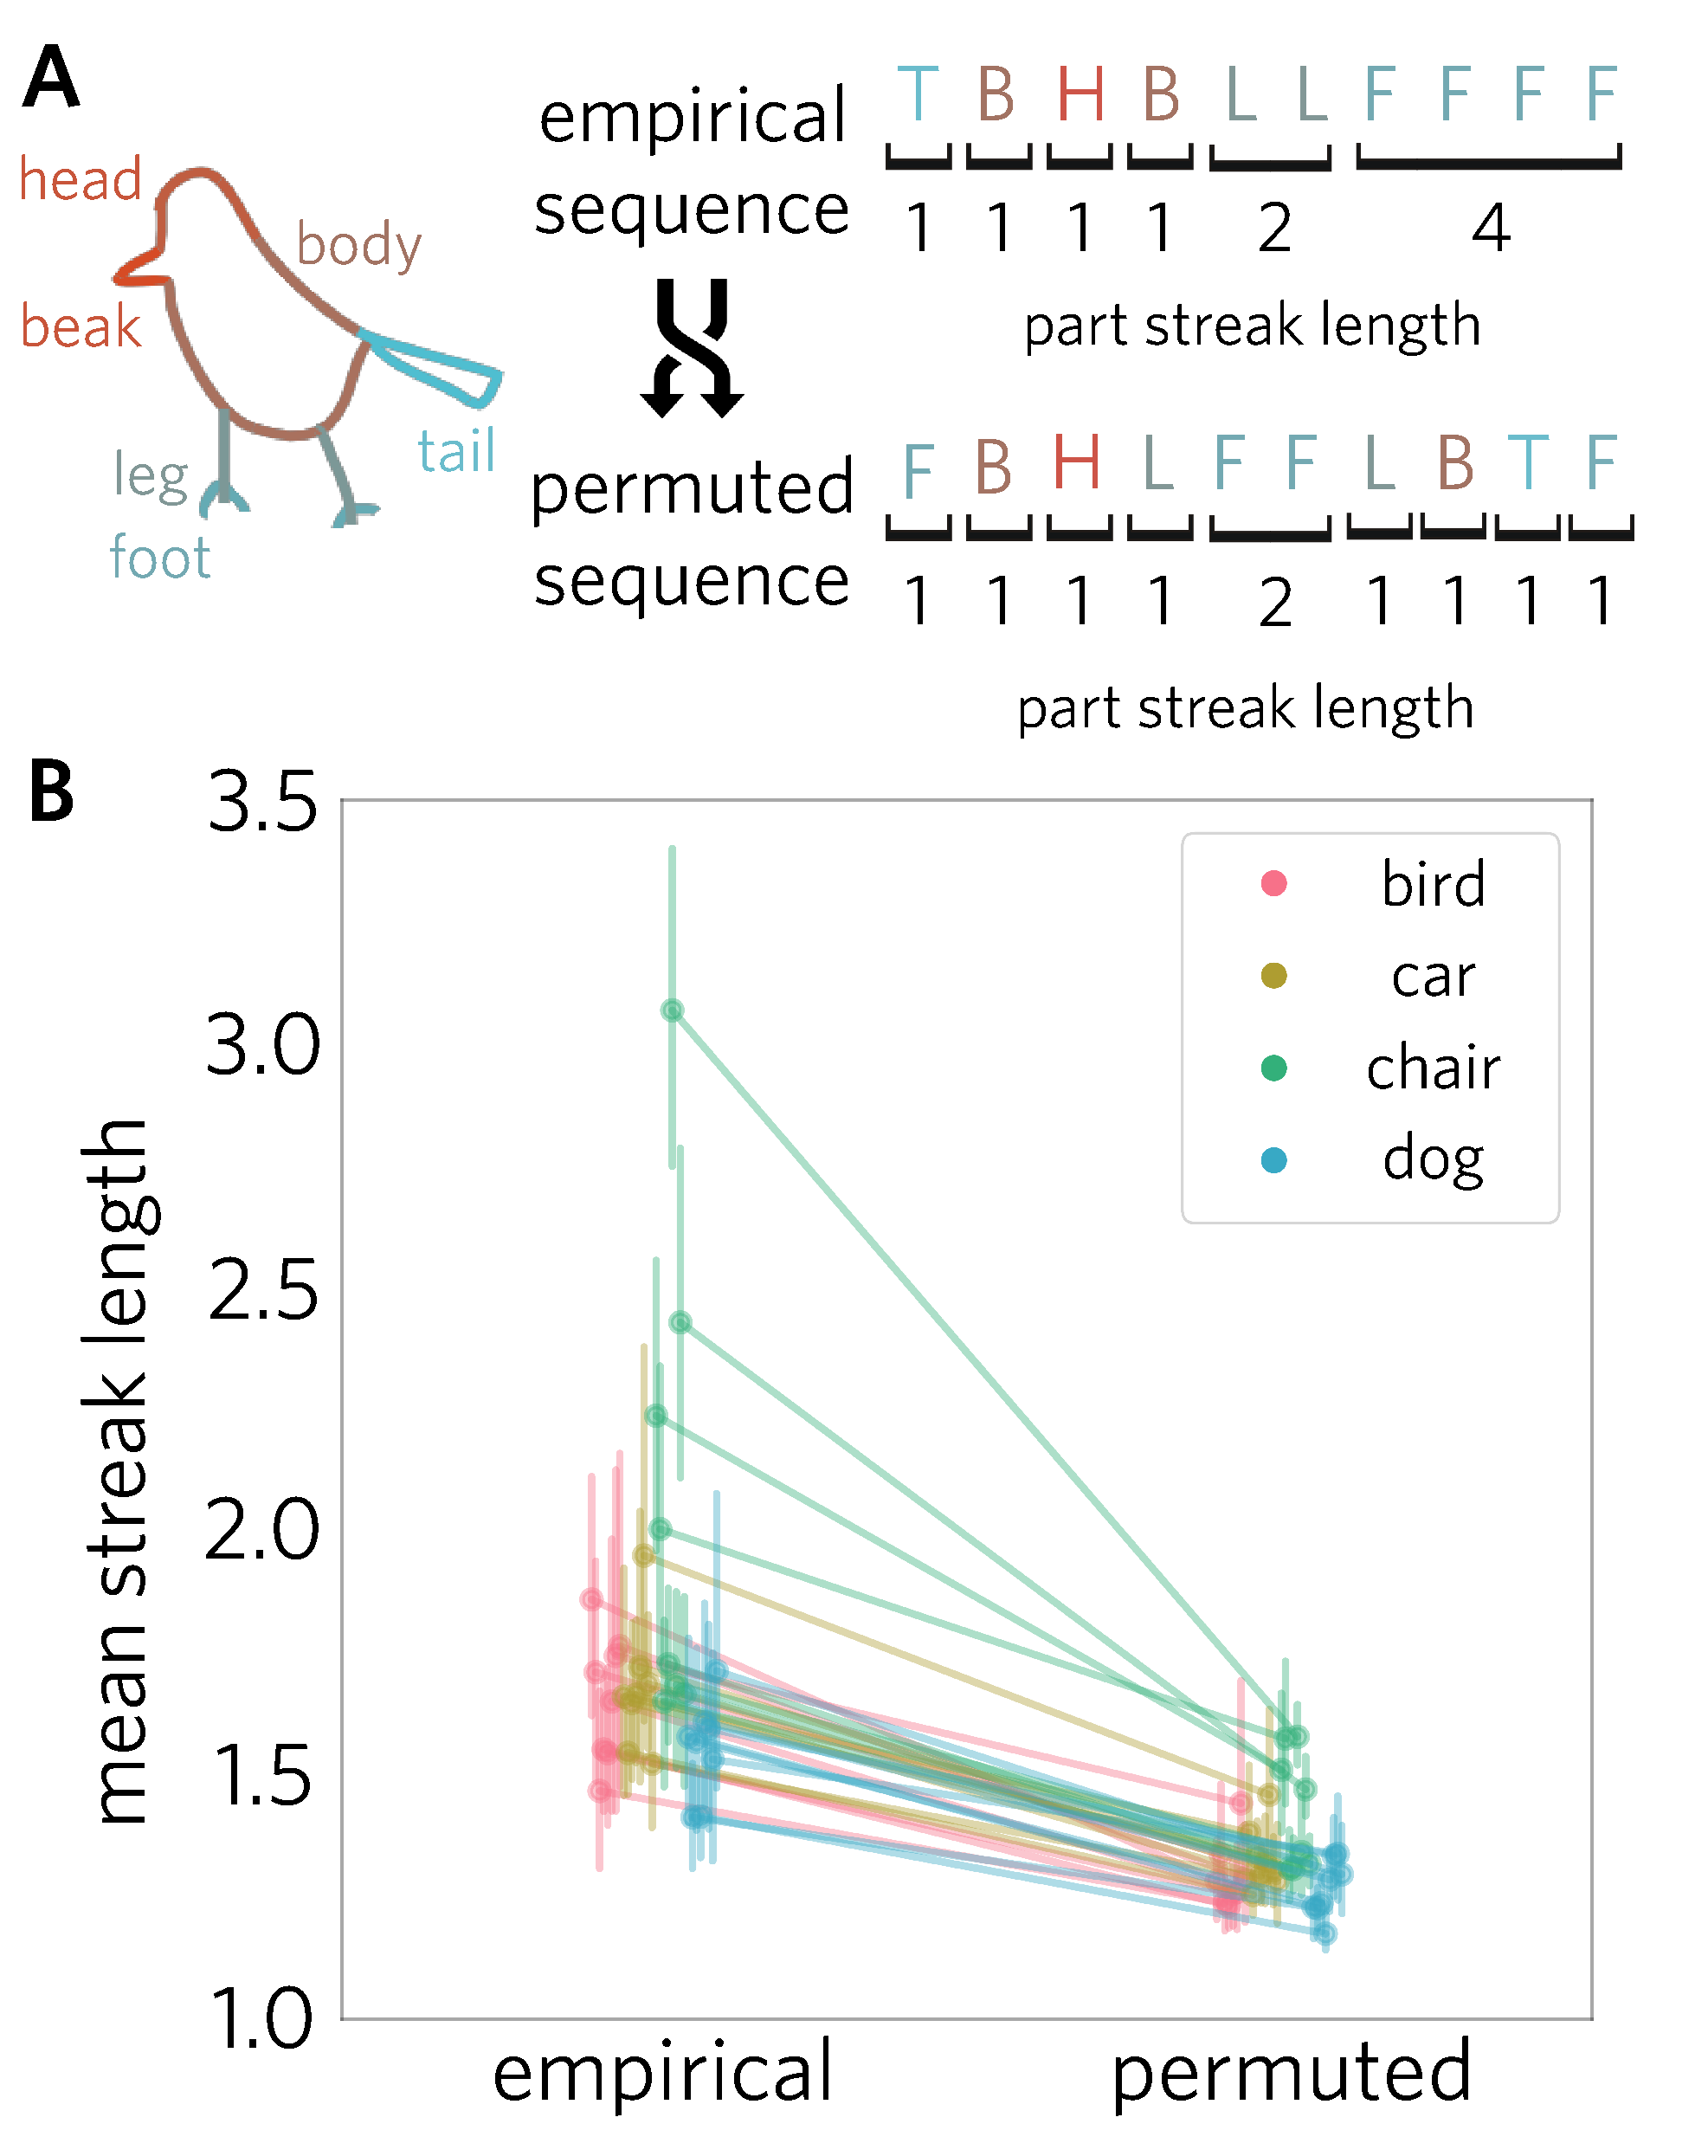
\includegraphics[width=0.45\textwidth]{figures/6_part_sequence.pdf}
\caption{(A) Analysis of sequence in which strokes depicting each part were drawn. (B) Comparison of mean length of streaks consisting of strokes that depict the same part with null distribution of permuted stroke sequences.}
\label{stroke_sequence_fig}
\end{figure}


To evaluate statistical reliability, we computed the z-score of the empirical streak length relative to the permuted streak length distribution for each sketch. 
This reflects the extent to which same-part strokes were clustered in time relative to a sequence with exactly the same distribution of strokes over parts, but in which strokes were produced in random order. If the empirical streak lengths were to be higher than the permuted streak lengths, it would indicate that not only do people's strokes tend to correspond to semantically meaningful parts, but that the sequence in which they make strokes to create drawings also reflects their knowledge of object-specific part structure. 
We found that the empirical streak length was reliably higher for all objects (z-score: 2.07, 95\% CI: [1.90, 2.23]), and higher for the close drawings (z-score: 2.58; 95\% CI: [2.26, 2.90]) than far drawings (z-score: 1.56; 95\% CI: [1.38, 1.74]).
Since close drawings tend to comprise of more strokes than far drawings, it is possible that these additional strokes serve to provide additional detail to parts in the sketch. If so, then parts are constructed at a finer compositional grain in close drawings, leading to a larger number of successive strokes of the same part.
All confidence intervals were estimated via stratified bootstrap resampling (N=1000 iterations) of drawings within object-context combinations.
Taken together, our results suggest that the procedure by which people convey semantic information when sketching is compositional: frequently, they use a single stroke to convey an entire part; but when they do use multiple strokes to convey a single part, they tend to draw these in succession before moving on to a different part. 

\begin{figure}[ht]
\centering
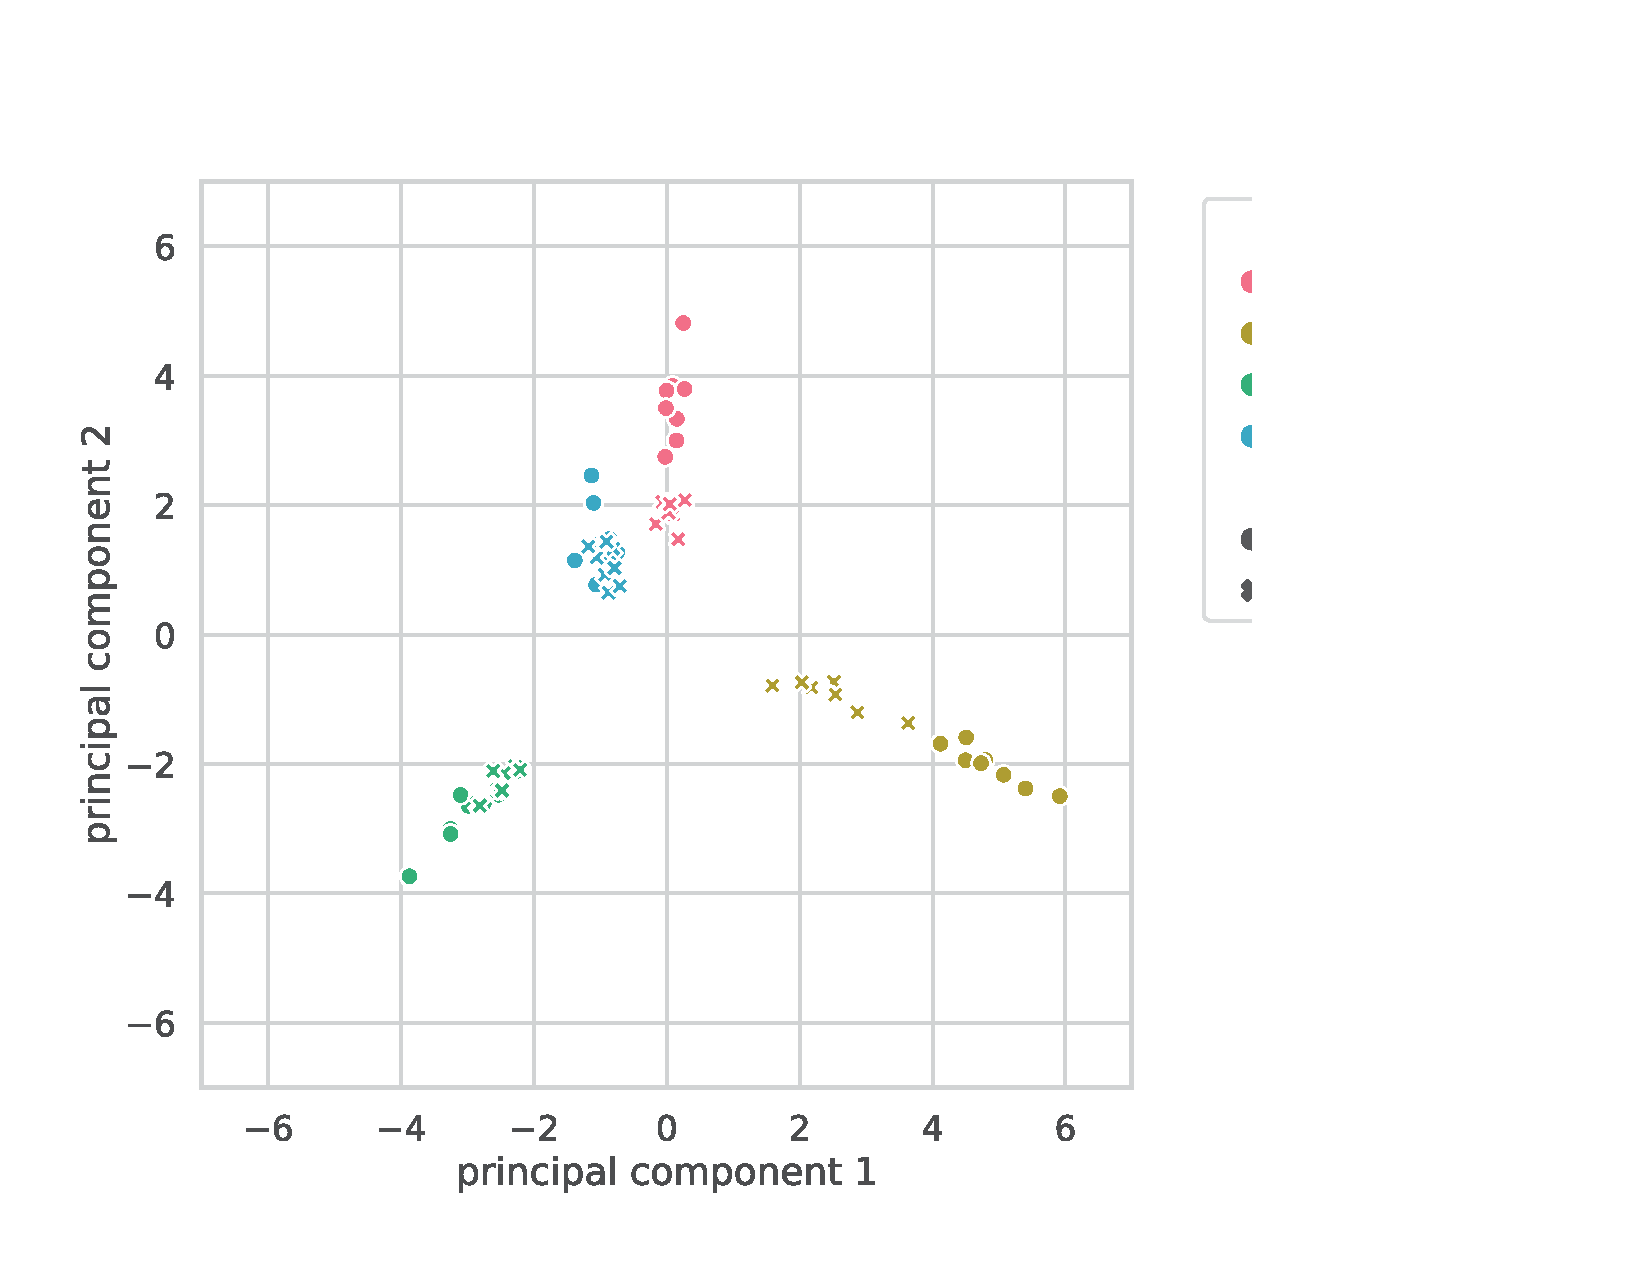
\includegraphics[width=0.4\textwidth]{figures/7_part_emphasis.pdf}
\caption{(A) Visualization of the distribution of mean feature vectors for each object-condition combination, projected onto the top two principal components. (B) Feature vectors of close and far drawings of the same object were more similar to each other than those of close and far drawings of different objects within a category. (C) Far drawings were more similar to each other than close drawings were to each other. *** indicates \textit{p}$<0.001.$}
\label{part_emphasis}
\end{figure}

\subsection{How is part information emphasized in different communicative contexts?}

Our findings so far bear on how the way people compose communicative drawings of objects reflects their semantic knowledge of which parts objects are composed of. 
A key consequence of such semantically organized part knowledge is that it naturally supports flexible expression across different communicative contexts. 
For example, when communicating about a chair in a (far) context containing objects from other basic-level categories, drawers may include only the essential information to indicate the presence of certain parts that distinguish it at the category level. 
On the other hand, when communicating about that same chair in a (close) context containing other, perceptually similar chairs, drawers may emphasize certain distinctive parts (e.g., the number of back slats) that distinguish it at the object level, by applying more strokes and/or more ink in each stroke.

We hypothesized that drawers emphasize part information across such communicative contexts in such a way that it preserves these relevant distinctions. 
To explore this possibility, we asked the following questions: 
(1) How similarly is object-specific part information emphasized in close and far communicative contexts? 
% (2) To the extent close and far drawings of the same object emphasize part information differently, does this reflect large differences in emphasis on a few parts, or small differences in emphasis across many parts? 
(2) How do differences in how part information is emphasized in close and far contexts affect how discriminable they are?

To investigate these questions, we represented each sketch by a \textit{part-feature vector} that combined information about: (a) how many strokes and (b) how much total ink was expended on each part of that object. 
In order to represent all drawings in our dataset using a common feature representation, we combined part labels across categories, yielding a set of 24 unique part labels to which any stroke could be assigned. 
Each part-feature vector thus consisted of 48 elements: 24 of these represented the number of strokes allocated to each part, and the remaining 24 represented the total arc length of all strokes allocated to each part. 
Before further analysis, we z-scored values within each feature dimension in order to map stroke count and arc length measurements to the same unit-variance scale. 
Because our primary goal was to understand differences between objects and contexts, we then collapsed across drawings within each object-context combination, yielding 64 average part-feature vectors (i.e., 32 objects x 2 context conditions). 

\subsubsection{Similar part profile across different communicative contexts}

In order to investigate to what extent similar object-specific part information is emphasized in different communicative contexts, we computed the matrix of Pearson correlations between part-feature vectors. 
Formally, this entailed computing: $R_{ij} =  \nicefrac{cov(\vec{r}_{i}, \vec{r}_{j})}{\sqrt{var(\vec{r}_{i}) \cdot var(\vec{r}_{j})}}$, where $\vec{r}_{i}$ and $\vec{r}_{j}$ are the mean part-feature vectors for the $i$th and $j$th object-context combinations, respectively.
If similar object-specific part information is emphasized in both contexts, this would yield higher correlations between close and far part-feature vectors for the \textit{same} object than for close and far part-feature vectors of \textit{different} objects. 
Consistent with this, we found that close and far drawings of the same object emphasized similar part information (within-object: $r = 0.740$, 95\% CI: [0.726, 0.753]), and to a greater degree than did close and far drawings of different objects (between-object: $r = 0.653$, 95\% CI: [0.646, 0.659]), suggesting that these patterns of emphasis were to some extent object-specific (Fig.~\ref{part_emphasis}B). 

% \subsubsection{Greater emphasis on a few parts when producing detailed drawings}

% Although the patterns of emphasis on different parts were similar between close and far drawings, close drawings expressed more part information overall.
% To what extent do close drawings accomplish this by placing a lot more emphasis on a few parts, or placing a little extra emphasis on many parts?
% To address this question, we first calculated the vector difference between the close and far part-feature vectors for each object.
% % To provide a geometric intuition, each difference vector represents the direction and distance to move in this 48-dimensional feature space to get from the centroid of the far drawings of an object to the centroid of its close drawings. 
% If close drawings place a lot more emphasis on a few parts, this difference vector will be sparse, containing a few large non-zero values and many zero values. 
% On the other hand, if close drawings tend to place a little extra emphasis on many parts, this difference vector will not be non-sparse, containing many similar non-zero values and few zero values. 
% We used the following metric to compute the sparsity of each difference vector:
% $\texttt{s}= \nicefrac{(\sqrt{k} - \frac{\norm{v}_1}{\norm{v}_2})}{(\sqrt{k}-1)}$, where $k=48$ (the dimensionality of the vector), $v$ is the difference vector, $\norm{v}_1$ is the L1-norm and $\norm{v}_2$ is the L2-norm. 
% Here, $s=1$ for maximally sparse vectors (i.e., single non-zero value) $s=0$ for minimally sparse vectors (i.e., all values identical and non-zero).
% We found that difference vectors were moderately sparse ($s=0.675$, 95\% CI: [0.653, 0.686]), suggesting that close drawings place more emphasis on a few different parts relative to far drawings, but not to the same extent for all parts (Fig.~\ref{part_emphasis}C).

\subsubsection{Detailed drawings are more distinct from each other than sparser drawings}

The above findings show that close drawings exhibited similar patterns of emphasis on different parts as their far counterparts. 
However, given that close drawings contain greater emphasis on these parts overall than far drawings (i.e., contain more and longer strokes), a natural question affect how this influences how discriminable they are.
\jefan{Kushin, I think we should report the basic observation that close drawings consist of more strokes and higher arclengths than far, with CIs, around here.}
We hypothesized this overall greater part information enhances the discriminability of close drawings from one another, relative to far ones, by increasing the feature distance between objects that otherwise share many perceptual properties. 
To evaluate this possibility, we compared the mean correlation distance (i.e., $1 - r$) between the part-feature vectors of close drawings of objects in a given category with that between far drawings of exactly the same objects. 
We found that close drawings were indeed reliably more distant from one another than far drawings were (close similarity: $r = 0.666$, 95\% CI: [0.652,685]; far similarity: $r = 0.729$, 95\% CI: [0.719,0.746]), suggesting that drawers discern which part information is most diagnostic of the target object among highly similar distractors, and emphasize this distinctive information accordingly (Fig.~\ref{part_emphasis}A \& C).

\section{Discussion}

We show here that people are highly consistent in what parts they interpret drawings' constituent strokes as representing. 
When the sequential strokes that a drawer produces to create a drawing are coded in terms of these parts, we see that there is a prevalent one-to-one correspondence between individual strokes and parts. 
We also observe that it is common for strokes representing the same part to be drawn in succession.
We take these results to support the idea that people's semantic knowledge of objects helps guide their decisions on what to depict through their strokes and how to organize these strokes in time.
The structure of completed drawings reflect this semantic part knowledge, even when drawings are produced in different contexts to varying degrees of detail. Detailed drawings of objects distinguish themselves from their sparser counterparts by preferentially expressing object-specific parts through their constituent strokes. However, both detailed and sparse drawings of objects preserve elements that help distinguish them from sketches of other objects.

By focusing on the number and length of strokes as well as their sequence, we are able to study the correspondence between observable semantic structure in sketches and the decisions drawers make to express this structure graphically.
And these decisions reveal to us that people are able to decompose an abstract object into part-categories and reconstruct it in a flexibly structured manner during graphical production. The flexibility is in modulating which parts to express to what degree, given the contextual needs of communication.
Our findings support the idea of compositionality in abstract visual conceptions of objects and categories. [LAKE ET AL 2017, BIEDERMAN 1987]. 
Such a form of representation is powerful for categorizing novel objects, discerning object identity through sparse or noisy channels, \kushin{too vague maybe?} and expressing concepts cheaply, as we see in the sparse drawings in our reference game dataset. 
Compositional organization of semantically meaningful components in varied relationships to each other allows for an adaptive perceptual system that is nevertheless sensitive to the prevalence of commonly occurring elements in our environment [GOLDSTONE 2003]. 

Taken as a whole, these results show that drawings reveal people's conceptual knowledge of objects through how components of the object are expressed through strokes. We show that by considering the number of strokes and amount of effort expended in producing each stroke we are able to account for how drawings are able to flexibly convey information across different communicative contexts. Future work will look to investigate the properties of the parts that these strokes represent, i.e., the quality of the content they express over just the quantity and organization of semantically meaningful parts. This would allow us to understand how the perceptual properties of objects and parts influence this semantic decomposition

\kushin{need to tighten this paragraph to have a narrative throughline}

%While our findings show that people's semantic knowledge of parts may influence how they recognize and produce drawings, we believe our current part-feature characterization to be an overly explicit instantiation of semantics in communicative drawings. Though we believe such approximations are beneficial to showing how modulating semantically meaningful information in drawings allows for flexibility in communication, we are yet to account for how perceptual properties of strokes in drawings are perceived as components that hold meaning for us. Thus, we are still shy of being able to translate the high dimensional feature spaces in modern vision models to more human-like perceptual representations through this approach alone. Future work will seek to integrate these two approaches.

\jefan{a thought to be fleshed out more: all the more remarkable we can extract these things based purely on considering something like effort cost // number of actions across categories. Future work should focus on extending this approach to consider the \textit{content} allocated to each part category, over and above \textit{quantity.}}
 

\section{Acknowledgments}
%Hide for now since blinded

%KM was supported by the Department of Cognitive Science at Vassar College through its Humanities in Cognitive Science program.
%RXDH was supported by the National Science Foundation Graduate Research Fellowship (DGE-114747). 

%\section{References}

\bibliography{semantic_parts}
\bibliographystyle{apacite}
\setlength{\bibleftmargin}{.125in}
\setlength{\bibindent}{-\bibleftmargin}ı






\end{document}
